\section{Related Work}
\label{sec:related}


\mypara{3D shape segmentation.}
Traditional 3D shape segmentation methods rely on fully supervised learning from part-annotated datasets such as ShapeNetPart~\cite{yi2016scalable}, PartNet~\cite{mo2019partnet}, and ScanObjectNN~\cite{uy2019revisiting}.
Early approaches focused on point-wise classification~\cite{Qi2016PointNetDL, Qi2017PointNetDH}, while later works explored prototype-based methods~\cite{He2020LearningAM, Yi2018GSPNGS} or co-segmentation objectives~\cite{Chen2019BAENETBA, Zhu2019AdaCoSegAS}.
Despite strong performance on known categories, these methods struggle to generalize to unseen objects and rely on costly manual supervision.
Scene-level segmentation methods~\cite{wu2024point} are more successful due to the amount of training data~\cite{Dai2017ScanNetR3, Yeshwanth2023ScanNetAH} and specialized networks~\cite{wu2024point} but cannot be directly applied to the more fine-grained domain of object-level part segmentation.
Our goal is to retain the feed-forward efficiency of supervised 3D models while enabling open-world part understanding.

\mypara{Adapting 2D foundation models to 3D.}
A parallel line of work explores the direct application of 2D foundation models, both uni-modal and language-vision models, to 3D by rendering point clouds from multiple views.
For scene segmentation, several works \cite{Nguyen2023Open3DISO3, 10655587, Peng2022OpenScene3S, Takmaz2023OpenMask3DO3} successfully extracted the 2D knowledge by projecting 2D features to 3D points. 
For shape analysis, PointCLIP~\cite{zhu2022pointclip} first showed that CLIP~\cite{radford2021learning} can perform zero-shot 3D classification from rendered images.
PointCLIPv2~\cite{zhu2022pointclip} further improves its performance and extends it to the more fine-grained task of part segmentation ,but with limited accuracy.
PartSLIP~\cite{liu2023partslip} adapted the GLIP~\cite{Li2021GroundedLP} bounding-box framework for object detection, while SATR~\cite{abdelreheem2023satr} refined this approach for mesh-based inputs.
Following the release of SAM~\cite{kirillov2023segment, ravi2024sam}, several works used it for class-agnostic 3D segmentation~\cite{Yang2024SAMPart3DSA, Liu2025PARTFIELDL3} with great success, and others combined it with 2D detectors for instance-level segmentation~\cite{Zhou2023PartSLIPEL, Xue2023ZeroPSHC}.
More recently, COPS~\cite{garosi20253d} used the powerful DINOv2~\cite{oquab2023dinov2} dense feature extractor to achieve state-of-the-art zero-shot shape segmentation results, though performance remains limited when using simple part text queries.
In contrast to these approaches, our method aims for a purely feed-forward 3D encoder that operates directly on point clouds.

\mypara{3D foundation models.}
Bridging the modality gap between 2D and 3D has led to the emergence of large-scale multimodal 3D foundation models.
ULIP~\cite{xue2023ulip} unified image, text, and 3D embeddings through cross-modal contrastive learning, while ULIP-2~\cite{xue2023ulip}, OpenShape~\cite{liu2023openshape}, and Uni3D~\cite{zhou2023uni3d} demonstrated that large-scale pre-training on Objaverse~\cite{deitke2023objaverse} enables strong zero-shot recognition.
However, these models primarily target global shape understanding rather than the more fine-grained part reasoning.
DITR~\cite{zeid2025dino} and OV3D~\cite{he2024unim} showed that distilling 2D features into a 3D encoder yields powerful geometric representations for scene segmentation,
while PartDistill~\cite{Umam2023PartDistill3S} attempted a similar strategy to one shape category at a time but with limited generalization across categories.
Find3D~\cite{ma2025find} advanced this direction by curating a 30K-shape Objaverse subset using SAM~\cite{kirillov2023segment} and Gemini~\cite{team2023gemini} captions to train an open-world feed-forward model.
Despite its scalability, Find3D still produces imprecise part boundaries and struggles with simple shapes.
Our work builds upon this data curation setup and introduces a two-stage pre-training framework that first transfers dense 2D features to 3D patches, then aligns them with language, achieving open-world, feed-forward part segmentation without any rendering at inference time.


\begin{figure*}[t]
  \centering
  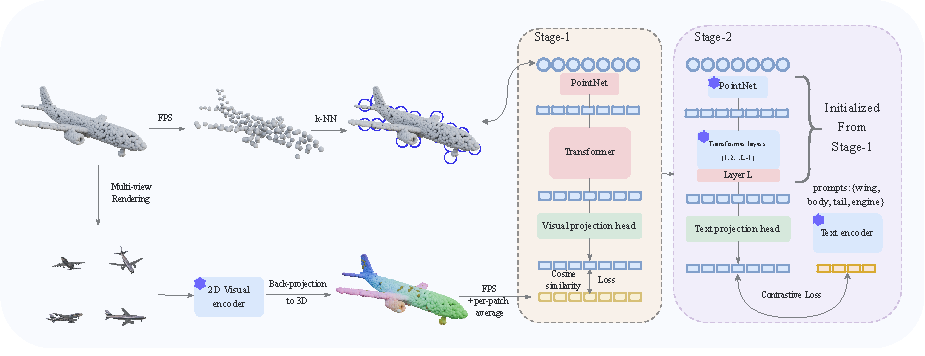
\includegraphics[width=\linewidth]{figs/method.pdf}
    \caption{\textbf{PatchAlign3D pre-training.}
    Given an input point cloud, we extract multi-view visual features using a 2D backbone
    and back-project them into 3D space. In \textbf{Stage 1},
    the 3D transformer encoder operates on sampled point cloud patches and learns to
    align its output patch tokens with the back-projected visual features. In \textbf{Stage 2},
    we initialize from Stage 1, freeze all earlier layers, and train only the last
    transformer block and projector to align patch-level features with textual embeddings
    in a contrastive manner.}
  \label{fig:arch}
\end{figure*}